\section{Math}
\subsection{Projections}
Projections are an important class of linear transformation. When we compress of visualize high-dimensionality data, we will lose information. To minimize this compression loss, we ideally find the most informative dimensions in the data.
\begin{definition}[Projection]
    Let V be a vector space $U \subseteq V$ a subspace of V. A linear mapping $\pi: V \longrightarrow U$ is called a projection if $\pi^2 = \pi \circ \pi = \pi$.
\end{definition}
A projection, in general, means concentrating on a particular direction, feature, set of features. Since the projection $\pi$ is a linear mapping and they can be expressed by transformation matrix there esists a transformation matrix $P_\pi$ such that $ P_\pi^2 = P_\pi $
\subsubsection{Projection onto one-dimensional subspaces}
\begin{definition}[Projection onto one-dimensional subspaces (lines)]
    Assume we are given a line (a one-dimensional subspace) through the origin with basis vector $b\in \mathbb{R}^n$. The line is a one-dimensional subspace $U\subseteq \mathbb{R}^n$ spanned by b. When we project $x \in \mathbb{R}^2$ onto U, we seek the vector $\pi_U(x) \in U$ that is closest to x. 
\end{definition}
\begin{figure}[htbp]
    \centering
    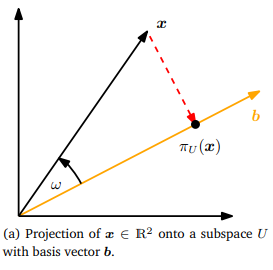
\includegraphics[width = 7cm]{Math/projectin_onto_line.png}
\end{figure}
Properties of the projection $\pi_U(x)$:
\begin{itemize}
    \item The projection $\pi_U(x)$ is closest to x, where "closest" implies that the distance $ \norm{vec x - \pi_u(vec x)} $ is minimal. It follows that the segment $\pi_U(x) -x$ from $\pi_U(x)$ to x is orthogonal to U, and therefore the basis vector b of U.
    \item The projection $\pi_U(x)$ of x onto U must be an element of U and, thereforre, a multiple of the basis vector b that spans U. Hence, $\pi_U(x) = \lambda b$, for some $\lambda \in \mathbb{R}$.
\end{itemize}
In the following three steps, we determine the coordinate $\lambda$, the projection $\pi_u(x) \in U$ and the projection matrix $P_\pi$ that maps any $x \in \mathbb{R}^n$ onto U.
\begin{enumerate}
    \item Finding the coordinate lambda. The orthogonality condicion yields
    \[ 
        \anglepar{x-\pi_U(x),b}= 0 \overset{\pi_U(x)=\lambda b}{\Longleftrightarrow } \anglepar{x-\lambda b, b} = 0
    \]We can now exploit the bilinearity of the inner product and arrive at
    \[ 
        \anglepar{x,b} -\lambda \anglepar{b,b}=0 \Longleftrightarrow \lambda = \frac{\anglepar{x,b}}{\anglepar{b,b}} = \frac{\anglepar{b,x}}{\norm{b}^2} 
    \]In the last step, we exploited the fact that inner products are symmetric. If we chose $\anglepar{\cdot,\cdot}$ to be the dot product, we obtain
    \[ 
        \lambda = \frac{b^Tx}{b^tb}= \frac{b^Tx}{\norm{b}^2} 
    \]If $\norm{b}=1$, then the coordinate $\lambda$ of the projection is given by $b^Tx$.
    
    \item Second step is always easy $ \pi_U(x) = \lambda b = \frac{\anglepar{x,b}}{\norm{b}^2}b = \frac{b^tx}{\norm{b}^2}b $ 
    \item Just rewrite to determine a matrix such that $ \pi_U(x) = P_\pi x$ we see that $P = \frac{b b^T}{\norm{b}^2} $ 
\end{enumerate}
\subsubsection{Projection onto general subspaces}
In the following we look at orthogonal projections of vectors $x \in \mathbb{R}^n$ onto lower-dimensional subspaces $U\subseteq \mathbb{R}^n$ with $\dim(U) = m \geq 1$. Assume that $(b_{1}, \ldots,b_{m})$ is an ordered basis of U. As for the one-dimensional case, we follow a three-step procedure. 
\begin{enumerate}
    \item Find the coordinates $\lambda_{1}, \ldots,\lambda_{m}$ of the projection (with respect to the basis of U), such that the linear combination
    \begin{align*}
        \pi_U(x) = \sum_{i=1}^{m}{\lambda_ib_i= B\lambda}\\
        B = [b_{1}, \ldots,b_{m}] \in \mathbb{R}^{n\times m}, \quad \lambda = [\lambda_{1}, \ldots,\lambda_{m}]^T \in \mathbb{R}^m
    \end{align*}
    is closest to $x \in \mathbb{R}^n$. Again, closest refers to minimum distance which means that the vector connecting $\pi_U(x) \in U$ and $x\in \mathbb{R}^n$ must be orthogonal to all basis vectors of U.
    After some more considerations we get the normal equation $\lambda = (B^TB)^{-1}B^Tx$, where $(B^TB)^{-1}B^T$ is called the psuedo inverse of B (which is not square). It can always be computed if BTB is invertible, this is true since B is a basis for U.
    \item Find the projection $\pi_U(x) \in U$ We already established that $\pi_U(x)=B\lambda$. Therefore
    \[ 
        \pi_U(x) = B(B^TB)^{-1} 
    \]
    \item Find the projection matrix $P_\pi$. From 2 we can immediately see that the projection matrix that solves $P_\pi x=\pi_U(x)$ must be 
    \[ 
        P_\pi=B(B^TB)^{-1}B^T 
    \]
\end{enumerate}
Projection is a tool for finding approximate solutions (by deleting some solutions). Projecting is easier when the base is orthonormal because BTB = I. Through Gram-Schmidt Orthogonalization we can turn any basis into an orthonormal one, going one dimension at a time.

\subsection{Matrix Decomposition}
\begin{figure}[htbp]
    \centering
    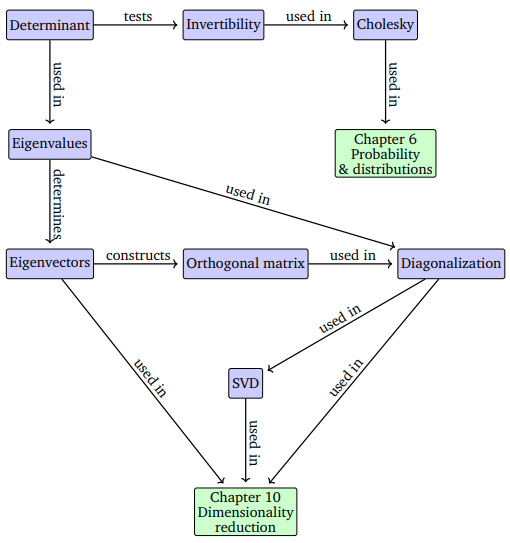
\includegraphics[width=10cm]{Math/matrix-decomposition-map.png}
\end{figure}
\subsubsection{Determinant and Trace}
The determinant of a square matrix A is a function that sends the matrix to a real number. A square matrix A is invertible if and only if $\det(A)= 0$ , this means that $rk(A)=n$. Two vectors in $\mathbb{R}^2$ are linearly independent if and only if they form a proper parallelogram.
\begin{theorem}[Laplace Expansion]
    Consider a matrix $A \in \mathbb{R}^{n\times n}$. Then, for all $j = 1, \ldots,n$:
    \begin{enumerate}
        \item Expansion along column j
        \[  
            \det(A) = \sum_{k=1}^{n}{(-1)^{k+j}a_{kj}\det(A{k,j})}  
        \]
        \item Expansion along row j
        \[  
            \det(A) = \sum_{k=1}^{n}{(-1)^{k+j}a_{jk}\det(A{j,k})}  
        \]
    \end{enumerate}
    Here $A_{k,j} \in \mathbb{R}^{(n-1)\times (n-1)}$ is the submatrix of A that we obtain when deleting row k and column j.
\end{theorem}
For $n=3$ the Sarrus'rule helps us calculate the determinant:
\begin{align*}
    \begin{bmatrix}
        a_{11} & a_{12} &a_{13}\\
        a_{21} & a_{22} &a_{23}\\
        a_{31} & a_{32} &a_{33}
    \end{bmatrix} &= a_{11}a_{22}a_{33}+a_{21}a_{32}a_{13}+a_{31}a_{12}a_{23}\\
    &-a_{31}a_{22}a_{13}-a_{11}a_{32}a_{23}-a_{21}a_{12}a_{33}
\end{align*}
For a triangular matrix $T \in \mathbb{R}^{n\times n}$, the determinant is the product of the diagonal elements
\[ 
    \det(T) = \Pi_{i=1}^{n}{T_{ii}} 
\]
The following are some of the properties of determinants:
\begin{itemize}
    \item The determinant of a matrix product is the product of the corresponding determinants, $\det(AB) = \det(A)\det(B)$
    \item Determinants are invariant to transposition, $det(A) = det(A^T)$
    \item If A is regular (invertible), then $\det(A^{-1})= \frac{1}{\det(A)}$
    \item Similar matrices possess the same determinant and the determinant is invariant to the choice of basis for the linear mapping
    \item Adding a multiple of a column/row to another one does not change $\det(A)$
    \item Swapping two rows/columns changes the sign of the determinant
\end{itemize}
\begin{definition}[Trace of a matrix]
    The trace of a square matrix $A \in \mathbb{R}^{n\times n}$ is defined as
    \[ 
        tr(A) = \sum_{i=1}^{n}{a_{ii}} 
    \]
    the trace is the sum of the diagonal elements of A and it satisfies the following properties:
    \begin{itemize}
        \item $tr(A+B) = tr(A) + tr(B), \quad A, B \in \mathbb{R}^{n\times n}$
        \item $tr(\alpha A) = \alpha tr(A)$
        \item $tr(I_n) = n$
        \item $tr(AB) = tr(BA), \quad A \in \mathbb{R}^{n\times k}, B \in \mathbb{R}^{k\times n}$
    \end{itemize}
\end{definition}
\begin{definition}[Characteristic Polynomial]
    For $\lambda \in \mathbb{R}$ and a square matrix $A \in \mathbb{R}^{n \times n}$
    \begin{align*}
        p_A(\lambda)&:= \det(A-\lambda I)\\
        & c_0 + c_1\lambda + c_2\lambda^2+ \cdots + c_{n-1}\lambda^{n-1}+(-1)^n\lambda ^n
    \end{align*}
    $c_{1}, \ldots,c_{n-1} \in \mathbb{R}$, is the characteristic polynomial of A. In particular
    \begin{align*}
        c_0 & = \det(A)\\
        c_{n-1} & = (-1)^{n-1} tr(A)
    \end{align*}
\end{definition}
\subsubsection{Eigenvalues and Eigenvector}
\begin{definition}[Eigenvalue and Eigenvector]
    Let $ A \in \mathbb{R}^{n\times n}$ be a square matrix. Then $\lambda \in \mathbb{R}$ is an eigenvalue of A and $x\in \mathbb{R}^n\setminus{0}$ is the corresponding eigenvector of A if
    \[ 
        Ax = \lambda x 
    \]
    We refer to this equation as the eigenvalue equation.
\end{definition}
\begin{theorem}
    $\lambda in \mathbb{R}$ is an eigenvalue of $A \in \mathbb{R}^{n\times n}$ if and only if $\lambda$ is a root of the characteristic polynomial $p_A(\lambda)$ of A.
\end{theorem}
\begin{definition}[Algebraic multiplicity]
    Let a square matrix A have an eigenvalue $\lambda_i$. The algebraic multiplicity of $\lambda_i$ is the number of times the root appears in the characteristic polynomial. 
\end{definition}
\begin{definition}[Eigenspace and Eigenspectrum]
    For $A \in \mathbb{R}^{n \times n}$ the set of all eigenvectors of A associated with an eigenvalue $\lambda$ spans a subspace of $\mathbb{R}^n$, which is called the eigenspace of A with respect to $\lambda$ and is denoted by $E_\lambda$. The set of all eigenvalues of A is called the eigenspectrum, or just spectrum, of A
\end{definition}
\begin{definition}[Geometric multiplicity]
    Let $\lambda_i$ be an eigenvalue of a square matrix A. Then the geometric multiplicity of $\lambda_i$ is the number of linearly independent eigenvectors associated with $lambda_i$. In other words, it is the dimensionality of the eigenspace spanned by the eigenvectors associated with $\lambda_i$. 
\end{definition}
\begin{theorem}
    Given a matrix A Rmn we can always obtain a symmetric, positive semidefinite matrix S in Rnn by defining \[ 
        S : = A^TA 
    \]
    Remark: if rk(A) = n, then $S:=A^TA$ is symmetric, positive definite. 
\end{theorem}
\begin{theorem}
    The eigenvectors $x_{1}, \ldots,x_{n}$ of a matrix A in Rnn with n distinct eigenvalues $\lambda_{1}, \ldots,\lambda_{n}$ are linearly independent. 
\end{theorem}
This is the sense in which eigenvectors "decide" the linear mapping. 
\begin{theorem}[Spectral theorem]
    IF A in Rnn is symmetric, there exsists an orthonormal basis of the corresponding vector space V consisting of eigenvectors of A and each eigenvalue is real. 
\end{theorem}
this theorem tells us that A can be decomposed in $PDP^T$
\begin{theorem}
    The determinnnt of a matrix A in Rnn is the product of its eigenvalues:
    \[ 
        det(A) = \Pi_{i=1}^{n}{\lambda_i} 
    \]
    where $\lambda_i \in \mathbb{C}$ are (possibly repeated) eigenvalues of A
\end{theorem}
\begin{theorem}
    The trace of a matrix A in Rnn is the sum of its eigenvalues:
    \[ 
         tr(A) = \sum_{i=1}^{n}{\lambda_i}
    \]
\end{theorem}
Eigenvalues describe the transformation of volume/perimeter of a unit (hyper) cube.
Decompositions: we want to disassembly linear maps in order to keep only relevant information. here bases play an important role
\begin{theorem}[Cholesky decomposition]
    A symmetric, positive definite matrix A can be factorized into a product $A = LL^T$ where L is a lower-triangular matrix with positive diagonal elements.
    L is called the cholesky factor of A, and L is unique.
\end{theorem}
To find L we just need to spell out the constraint. Observation: all the elements of L are positive.
\begin{definition}[Diagonalizable]
    A matrix in Rnn is diagonalizable if it is similar to a diagonal matrix, i.e. if there exists an invertible matrix P in rnn such that $D = P^{-1}AP$
\end{definition}
Similar matrices are different descriptions of the same map. Diagonalizing A is equivalent to expressing the linear mapping in the base of eigenvectors. Use the eigenvectors for basis change (direction) and the eigenvalues for the diagonal matrix (stretching)
\[ 
    D =
    \begin{bmatrix}
        \lambda_1 & \cdots & 0 \\
        \vdots & \ddots & \vdots \\
        0 & \cdots & \lambda_n
    \end{bmatrix} 
    \quad P = (\vec{p}_{1}, \ldots,\vec{p}_{n})
\]
$AP = PD$ 
\begin{theorem}[Eigendecomposition]
    A square matrix A in Rnn can be factored into \[ 
        A = PDP^{-1} 
    \]
    where P in Rnn and D is a diagonal matrix whose diagonal entries tare the eigenvalues of A, if and only if the eigenvectors of A form a basis of Rn
    
\end{theorem}
\begin{theorem}
    A symmetric matrix S in Rnn can always be diagonalized
    \[ 
        S = PDP^{-1} 
    \]
\end{theorem}
Insert geometric picture, P fixes the direction and D fixes the lengths.\\
What if A is not square? 
\begin{theorem}[SVD theorem]
    Let A in Rmn be a rectangular matrix of rank $r \in [0,\min(m,n)]$. The SVD of A is a decomposition of the form

    with an orthogonal matrix U in Rmm with column vectors $u_i, i = 1, \ldots,m$ and an orthogonal matrix V in Rnn with column vectors $v_j, j = 1, \ldots,n$. Moreover, $\Sigma$ is an m x n matrix with $ \sum_{ii} = \sigma_i \geq 0$ and $\Sigma_{ij} = 0, i\neq j$ 
\end{theorem}
Geometrically it is as before but without "matching" domain-codomain dimensions. Insert picture and matrices 
\begin{definition}[Spectral norm of a matrix]
    For x in $Rn \setminus {0}$ the spectral norm of a matrix A in Rmn is defined as 
    \[ 
        \norm{A}_2 = \max_{x}{\frac{\norm{A}_2}{\norm{x}_2}} 
    \]
\end{definition}
\begin{theorem}
    The spectral norm of A is its largest singular value $\sigma_i$
\end{theorem}
\begin{theorem}[Eckart-Young Theorem]
    Consider a matrix A in Tmn of rank r and let B in Rmn be a matrix of rank k. For any $k\leq r$ with $\hat{A}(k) = \sum_{i=1}^{k}{\sigma_iu_iv_i^T}$ it holds that
    \begin{align*}
        \hat{A}(k) &= \argmin_{rk(B)=k}{\norm{A-B}_2}\\
        \norm{A-\hat{A}(k)}_2 &= \sigma_{k+1}
    \end{align*}
\end{theorem}